\begin{figure}[ht]
	\centering
	\footnotesize

	\psfrag{oh}[c][c] {$O$}

	\psfrag{u}[c][c] {$u$}
	\psfrag{fu}[c][c] {$f(u)$}

	\psfrag{fuR}[c][c] {$f(u_{R})$}
	\psfrag{fuL}[c][c] {$f(u_{L})$}
	\psfrag{fus}[c][c] {$f(u_{s})$}

	\psfrag{uR}[c][c] {$u_{R}$}
	\psfrag{uL}[c][c] {$u_{L}$}
	\psfrag{us}[c][c] {$u_{s}$}

	\psfrag{fpuR}[c][c] {$f'(u_{R})$}
	\psfrag{fpuL}[c][c] {$f'(u_{L})$}
	\psfrag{fpus}[c][c] {$f'(u_{s}) = 0$}

	\psfrag{cvLR}[c][c] {$\text{Convex: } u_{L} < u_{R}$}
	% \psfrag{cvRL}[c][c] {$\text{Convex: } u_{L} < u_{R}$}

	\psfrag{ccLR}[c][c] {$\text{Concave: } u_{L} > u_{R}$}
	\psfrag{ccRL}[c][c] {$\text{Concave: } u_{L} < u_{R}$}

	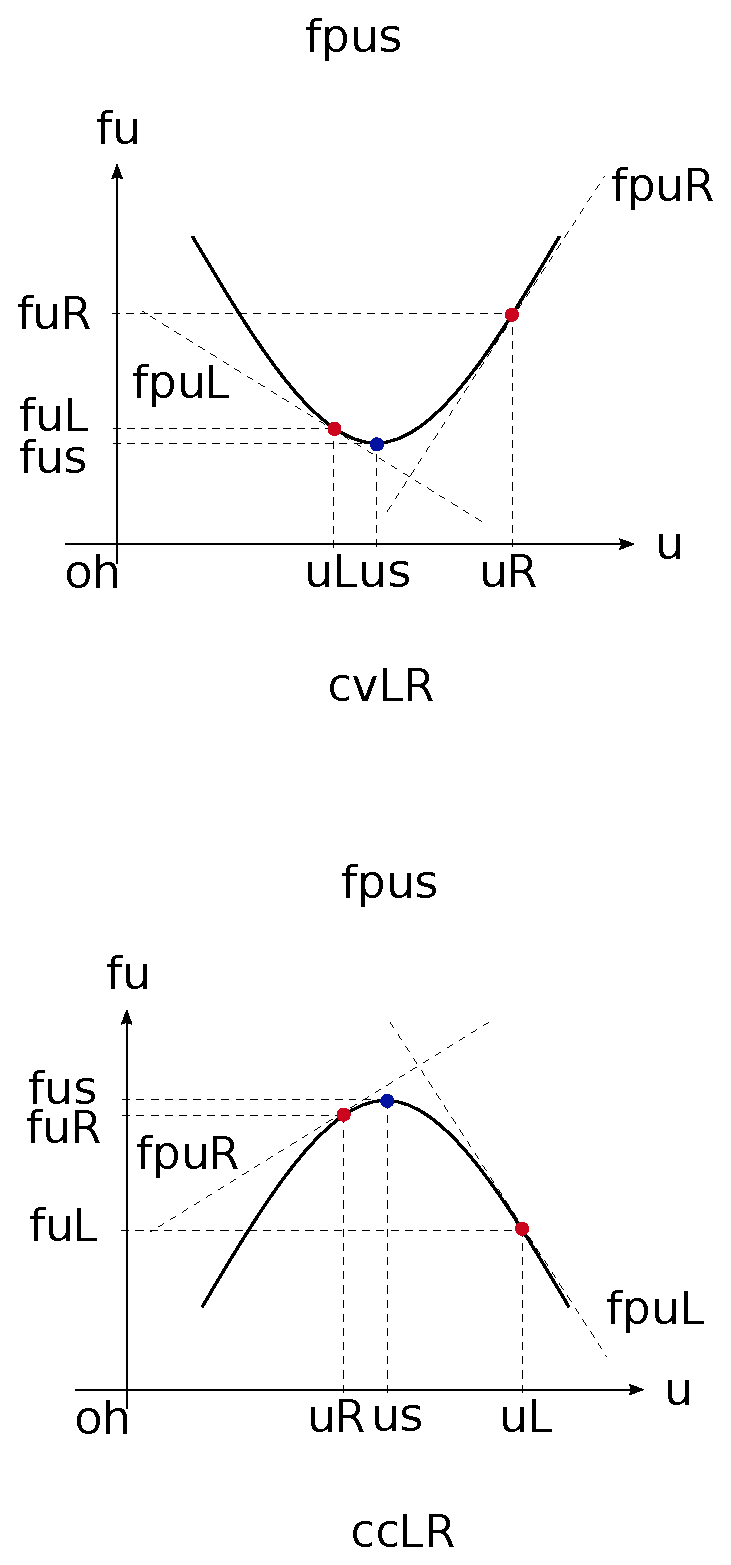
\includegraphics[width=0.7\textwidth]{convexityfu_case3.eps}
	\caption{Case 3:
		Convexity and concavity for $u_{L} < u_{R}$ and $u_{L} > u_{R}$,
		where the condition $f^\prime(u_L) < 0 <  f^\prime(u_R)$ holds.}
	\label{\LABEL}
\end{figure}